\documentclass{article}
\usepackage{tikz}
\begin{document}

A max-heap stored in an array $[90, 72, 65, 40, 31, 18, 7, 12]$:

\begin{center}
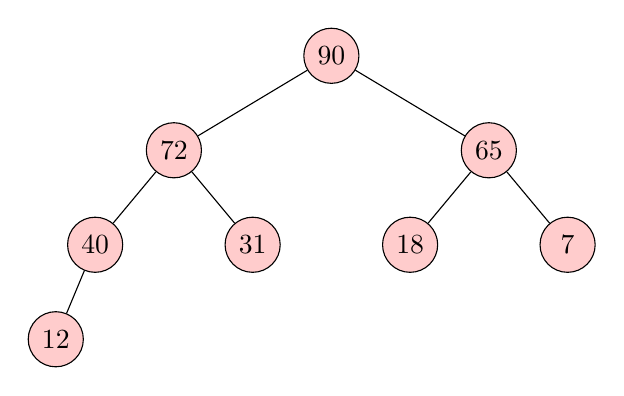
\begin{tikzpicture}[
  level 1/.style={sibling distance=4cm},
  level 2/.style={sibling distance=2cm},
  level 3/.style={sibling distance=1cm},
  level distance=1.2cm,
  every node/.style={circle, draw=black, fill=red!20, minimum size=7mm, inner sep=1pt}
]
\node {90}
  child {node {72}
    child {node {40}
      child {node {12}}
      child[missing]
    }
    child {node {31}}
  }
  child {node {65}
    child {node {18}}
    child {node {7}}
  };
\end{tikzpicture}
\end{center}

\end{document}
